\chapter{Benchmarks and Metrics in Industry}\label{ch:benchmarks_and_metrics}
In this chapter all the tools and the benchmarks for object localization and detection will be exposed. In particular, first the metrics and the techniques used to evaluate pose estimations will be presented, then some publicly available datasets will be presented. 

The problems that are going to be tackled are related to the 6D object pose estimation task. A 6D object pose is mathematically the 3D position of the object in the space plus 3 more terms that describe its rotation:

\begin{equation}
    \label{eq:6D_obj_pose_0}
    \hat{P} = (x, y, z, \alpha_x, \alpha_y, \alpha_z)^T
\end{equation}

The Eq. \ref{eq:6D_obj_pose_0} refers to the 6D pose estimate of an object, the first three terms $x, y, z$ describe the position in the camera reference frame, while the last three terms $\alpha_x, \alpha_y, \alpha_z$ represent the object's rotation angles along the $x, y, z$ camera axis respectively. This formulation can be easily manipulated in terms of rotation matrices and translation vectors:

\begin{equation}
    \label{eq:6D_obj_pose_1}
    \hat{P} = (R, t)
\end{equation}

The Eq. \ref{eq:6D_obj_pose_1} is a manipulated version of \ref{eq:6D_obj_pose_0} where the rotation matrix $R$ encodes the three angles of rotation $\alpha_x, \alpha_y, \alpha_z$ and the translation vector $t$ encodes the $x, y, z$ position of the object in the reference frame of the camera.

\begin{figure}
	\centering
	\begin{subfigure}{.5\textwidth}
  		\centering
  		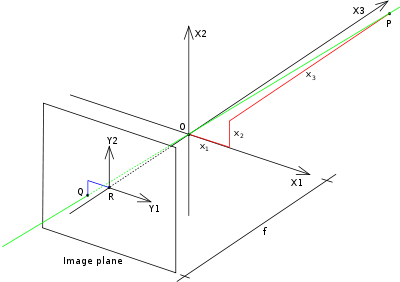
\includegraphics[width=.9\linewidth]{figures/2_benchmarks_and_metrics/pinhole_geometry_3D}
  		\caption{3D view}
  		\label{fig:pinhole_geometry3D}
	\end{subfigure}%
	\begin{subfigure}{.5\textwidth}
  		\centering
  		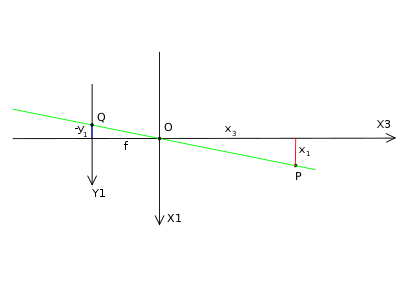
\includegraphics[width=.9\linewidth]{figures/2_benchmarks_and_metrics/pinhole_geometry_2D}
  		\caption{2D view}
  		\label{fig:pinhole_geometry2D}
	\end{subfigure}
	\caption{\textbf{Pinhole Camera Geometry.} In (A) the geometry of the pinhole camera in 3D view, in (B) its 2D representation.}
	\label{fig:pinhole_geometry}
\end{figure}

Each object pose estimate can also be projected back to the camera image plane. This projection between the 3D space and the 2D space of the image plane is achieved by applying the projection obtained with a given camera matrix model. The camera model that we consider here is the so called Pinhole Camera Model, and it's geometry is depicted in Figure \ref{fig:pinhole_geometry}.

The mapping from the coordinates of a 3D point $P$ to the 2D image coordinates of the point's projection onto the image plane, according to the pinhole camera model is given by:

\begin{equation}
    \label{eq:3D_to_2D_mapping}
    x_i = \left[ \begin{array}{c} u \\ v \end{array} \right] = \dfrac{f}{x_3} \left[ \begin{array}{c} x_1 \\ x_2 \end{array} \right]
\end{equation}

In Eq. \ref{eq:3D_to_2D_mapping} $x_1, x_2, x_3$ represent the 3D position in space of a generic point, $f$ is the focal length of the camera, and $u, v$ are the image coordinates obtained after the projection.

The formulation just explained is for an ideal pinhole camera located in the origin and with focal length equal for the $x$ and $y$ axes of the image. Typically, the situation is different, and the more generic formulation is like the following:

\begin{equation}
    \label{eq:generic_pinhole_camera_model}
    x_i = \left[ \begin{array}{c} u \\ v \\ 1 \end{array} \right] = \begin{bmatrix} f_x & 0 & c_x \\ 0 & f_y & c_y \\ 0 & 0 & 1 \end{bmatrix} \left[ \begin{array}{c} x_1 \\ x_2 \\ x_3 \end{array} \right]
\end{equation}

In Eq. \ref{eq:generic_pinhole_camera_model} the camera is formulated using its internal parameter $f_x, f_y, c_x, c_y$ that represent respectively the two focal lengths on the $x, y$ image axis and the camera optical center $(c_x, c_y)^T$.

With Eq. \ref{eq:3D_to_2D_mapping} and \ref{eq:generic_pinhole_camera_model} we can project each point of the 3D object model onto the image plane and compare the estimated pose with the ground truth one following one of the metrics that are going to be explained in the sections below.

\section{Metrics}\label{sec:metrics}
The problem of evaluating how good is a pose estimate w.r.t. the ground truth is a challenging and still very open topic in computer vision community.  Taking inspiration from \cite{hodan20166DPoseEstimation} we will first focus on bounding box estimates comparison and then will pass to the more complex and challenging problem of compare two object 6D pose estimate.

\begin{figure}
    \centering
    
\includegraphics[width=0.8\textwidth]{figures/2_benchmarks_and_metrics/placeholder800x600}
    \caption{\textbf{IoU score estimation example.} An eample of estimating the 2D bounding box of an object with the Halcon Libraries.} 
    \label{fig:iou_example}
\end{figure}

\subsection{2D Intersection over Union (IoU)}\label{subsec:iou}
The most common way to measure accuracy of object detection in 2D domain is to calculate the Intersection over Union score \cite{everingham2015challenge}:

\begin{equation}
    \label{eq:iou_score}
    s_{IOU}(\hat{B}, \bar{B}) = \dfrac{area(\hat{B} \cap \bar{B})}{area(\hat{B} \cup \bar{B})}
\end{equation}

In Eq. \ref{eq:iou_score} $\hat{B}$ and $\bar{B}$ are the estimated and ground truth 2D region respectively. Depending on the task, $\hat{B}$ and $\bar{B}$ can be rectangular regions (given by bounding boxes) or segmentation masks. For evaluation of 6D object pose estimates, the 2D regions can be obtained by projection of the object model $\mathit{M}$ in the estimated pose $\hat{P}$ and the ground truth pose $\bar{P}$ . Such pose error function is ambiguity-invariant, but since it operates in the projective space, it provides only a weak information about fitness of the object surface alignment. That basically means that every projection of the model that realizes in the same bounding box will have the very same score, even if the object is completely flipped among the two 6D poses. It is said that the IoU score is not ambiguity-invariant, we will see in the further section what ambiguity is. 

That is the reason why we only consider IoU for 2D measurement comparison, and so, only for object detection tasks, where just the location of the object within the image plane is considered to be interesting, not its exact position and orientation in 3D space. Examples of bounding boxes comparison, so IoU estimation is given in Figure \ref{fig:iou_example}. Usually a object detection is considered correct, when the IoU score of 2D bounding boxes of an object in the estimated and the ground truth pose is above a
threshold (e.g. 0.5).

\subsection{5cm, 5deg criteria}\label{subsec:5cm5deg}
After having introduced the metrics used for comparing object detection estimates, we now pass to tackle the problem of estimating the ``goodness'' of a 6D pose estimate. In the introduction of chapter \ref{ch:benchmarks_and_metrics} we formulated the pose of an object in 3D space in terms of rotation  matrix and translation vector, as stated in Eq. \ref{eq:6D_obj_pose_1}. From this simple formulation, intuitively, a simple error function can be built, in particular we can consider the error of the estimated pose $\hat{P} = (\hat{R}, \hat{t})$ w.r.t. the ground truth pose $\bar{P} = (\bar{R}, \bar{t})$ as composed by two independent terms, the translational error $(e_{TE})$ and the rotational error $e_{RE}$ respectively. These errors can be used as a metric for the computation of the goodness of a 6D pose estimate.

More in detail, the aforementioned $e_{TE}$ and $e_{RE}$ can be mathematically expressed as:

\begin{equation}
    \label{eq:translational_error}
    e_{TE}(\hat{t}, \bar{t}) = \norm{\hat{t} - \bar{t}}_2
\end{equation}

\begin{equation}
    \label{eq:rotational_error}
    e_{RE}(\hat{R}, \bar{R}) = arccos(\dfrac{Tr(\hat{R}\bar{R}^{-1}) - 1}{2})
\end{equation}

In particular, Eq. \ref{eq:translational_error} is simply the squared distance from the 2 points represented by their respective translation vectors $\hat{t}$ and $\bar{t}$, and Eq. \ref{eq:rotational_error} represents the rotational error in the axis-angle representation of the rotation matrices $\hat{R}$ and $\bar{R}$. More over, in $e_{RE}$, the function $Tr()$ is the trace of the rotation matrix.

After the previous formulation, we can now introduce a simple and intuitive criteria for evaluating the goodness of a 6D pose estimate. In \cite{shotton2013coordinate}, the so called \emph{5cm, 5deg} criteria have been introduced. It simply states that it is considered a good pose estimate if and only if $e_{TE} \leq 5cm$ and $e_{RE} \leq 5deg$. Of course, more general formulation of the same criteria can be used, by imposing variable thresholds $t_{TE}$ and $t_{RE}$ in the place of the constants $5cm$ and $5deg$.

This criteria was initially used for evaluating camera pose estimations, and it perfectly fits the case, but in terms of computing the goodness of a 6D object pose estimate, it is not adaptive to object model projections, in the sense that 2 different poses that refer to 2 different model projection onto the image plane can assume the very same $e_{TE}$ and $e_{RE}$, so those errors are still not ambiguity-invariant, as like as the IoU score.

\subsection{Pose Ambiguity Invariant Metrics}\label{subsec:pose_ambig_invariant_metrics}
Before introducing the idea of Average Distance for model points let's introduce the concept of \emph{Indistinguishable Poses} and \emph{Invariance to Pose Ambiguity}. As anticipated in the last two sections, IoU score and rotational and translational errors are not invariant to pose ambiguities, so let's see what this concern before introducing how we can overcome this issue.

\subsubsection{Indistinguishable Poses}\label{subsubsec:indistinguishable_poses}
If we take as example a generic object model, call it $M$, we can define a class of \emph{indistinguishable} poses for this model with the following:

\begin{equation}
    \label{eq:indistinguishable_poses}
    [P]_{M,I,\epsilon} = {P^{\prime} : d(v_I[PM], v_I[P^{\prime}M]) \leq \epsilon}
\end{equation}

where $v_I[M] \subseteq M$ is that part of the object model M that is actually visible in the image $I$, that is not self-occluded or occluded by some other object, $d$ is a distance between the surfaces, and $\epsilon$ is a threshold that basically controls the level of detail that we want to achieve in comparing two different views of the same model in the image.

\subsubsection{Invariance to Pose Ambiguity}\label{subsubsec:pose_ambiguity_invariance}
Pose Ambiguity is a necessary property for a 6D object pose estimator. Given an image $I$, a model $M$ and an estimated pose $\hat{P}$, the error $e(\hat{P}, \bar{P}; M, I)$ is required to be invariant under pose ambiguity iff:

\begin{equation}
    \label{eq:pose_ambiguity_invariance}
    \forall \hat{P}^\prime \in [\hat{P}]_{M, I, \epsilon},
    \forall \bar{P}^\prime \in [\bar{P}]_{M, I, \epsilon} : 
    e(\hat{P}^\prime, \bar{P}^\prime) \approx e(\hat{P}, \bar{P})
\end{equation}

where the approximation is given because of the $\epsilon$ tolerance term. A pose error function $e$ that satisfy such property is called \emph{ambiguity-invariant}.

This property is extremely important because an 6D object pose estimator relies its estimates only on the single image, there is no tracking information, and any other spatial relation with the model pose in the image that can distinguish two different pose estimates, so pose ambiguity cannot be removed in any way, that is why we need to model it somehow.

\subsubsection{Average Distance (AD)}\label{subsubsec:average_distance}
To do ...

\subsubsection{Visible Surface Distance (VSD)}\label{subsubsec:average_distance}
To do ...

\section{Industrially oriented Datasets}\label{sec:datasets}
To do ...

\subsection{T-LESS Dataset}\label{subsec:tless_dataset}
T-LESS Dataset \cite{hodan2017tless}.

\subsection{MVTec ITODD}\label{subsec:mvtex_itodd}
To do ...